% !TeX root = main.tex
\section{Method}
\label{sec:method}

CART transfers finger motion from a tactile glove to the 20-DoF Wuji2 hand. The policy predicts a sequence of joint updates from measured glove signals. During training, a calibrated human hand mesh provides geometric targets, and differentiable robot geometry maps contact and collision errors to joint-space gradients (Fig.~\ref{fig:cart-overview}).

\begin{figure*}[t]
    \centering
    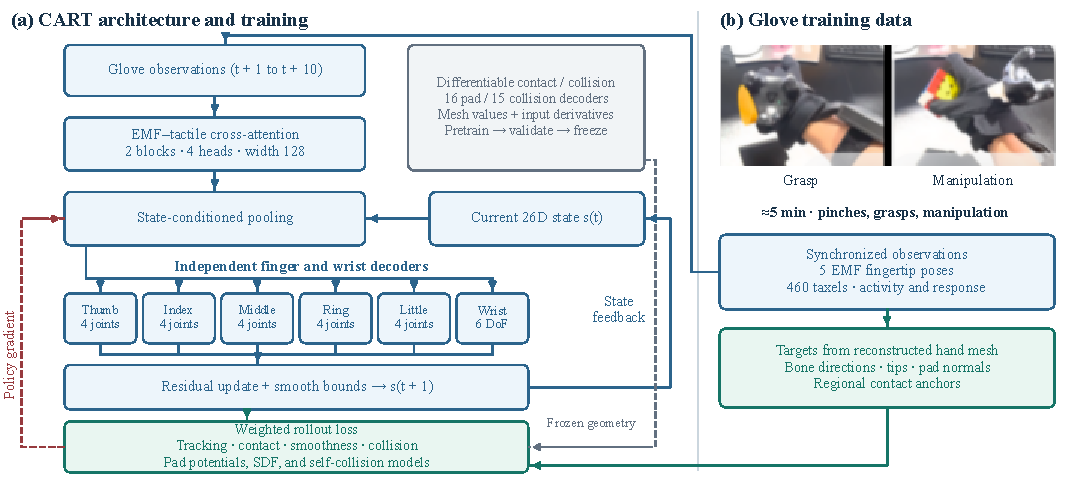
\includegraphics[width=\textwidth]{figs/cart_overview.pdf}
    \caption{CART architecture and training data. Left, five finger-specific decoders share an observation encoder. Weighted tracking, contact, smoothness, and collision losses backpropagate through the predicted states. Detached predictions provide native-mesh supervision for separate geometry updates. Right, synchronized glove signals and derived training targets. The photographs illustrate tactile-glove acquisition.}
    \label{fig:cart-overview}
\end{figure*}

\subsection{Network Architecture}
\label{sec:cart-architecture}

At step $t$, the policy receives the current robot joint angles $q_t$ and a window of ten measured glove frames, from $t+1$ through $t+10$. Each frame contains the electromagnetic (EMF) receiver pose for each of the five fingertips and the positions and binary contact states of 460 tactile elements (taxels). We express spatial observations in a canonical hand frame and represent each receiver rotation by its first two matrix columns. Relative timestamps encode the interval from the current robot state, and validity masks mark missing measurements. Online inference buffers the measured lookahead window before producing an update.

The encoder projects EMF and tactile inputs into 128-dimensional tokens and adds embeddings for frame index, relative time, and finger or taxel identity. Two four-head cross-attention blocks use the EMF tokens as queries and the tactile tokens as keys and values. Each head uses scaled dot-product attention with a mask for invalid keys. Each block applies residual connections around attention and its feed-forward layer. A further attention block uses an embedding of the current normalized joint state to pool the fused tokens into a shared representation. Five independent multilayer perceptrons, each with two 256-unit hidden layers, decode this representation into four joint increments per finger. Let $z_t$ denote the pooled context and $D_f$ the decoder for finger $f$. The normalized increment $\Delta\bar q_t$ concatenates the five outputs $D_f(z_t)$ in thumb-to-little-finger order. A $\tanh$ output bounds each increment. Let $\bar q$ denote joint angles rescaled to $[-1,1]$ using the robot's joint limits. The next state is given by
\begin{equation}
    \bar q_{t+1} = \operatorname{clip}
    \bigl(\bar q_t + \Delta\bar q_t,\,-1,\,1\bigr).
    \label{eq:cart-state-update}
\end{equation}
For joint $j$ with limits $(l_j,u_j)$, normalization uses $\bar q_{t,j}=2(q_{t,j}-l_j)/(u_j-l_j)-1$. Thus a decoder output has the same normalized range across joints, while its physical scale depends on the joint range. We map the clipped state back to radians for forward kinematics and feed it into the next update. The shared encoder lets a finger's decoder use observations from the other fingers.

\subsection{Hand Mesh Estimation}
\label{sec:cart-hand-mesh}

We reconstruct the demonstrator's hand using a skinned template driven by an articulated hand model. Six calibration poses comprise four thumb-to-finger pinches, a pose with the four finger bases flexed and the remaining joints extended, and a flat palm. We jointly fit finger bone lengths, the rigid receiver-to-distal-link transforms, and the transmitter-to-wrist transform. We compose the transmitter-to-wrist alignment, distal-link forward kinematics, and receiver mounting transform to predict each receiver pose in the transmitter frame. The fit uses measured EMF positions and orientations, contact and posture constraints from the calibration poses, and regularization on the fitted parameters. With these parameters fixed, we estimate hand joint angles frame by frame using joint-bounded inverse kinematics on the measured EMF poses.

Linear blend skinning deforms the template with the estimated joint angles. Each taxel is attached to a mesh triangle by fixed barycentric coordinates, so its position is $x_i=\sum_{k=1}^{3}\beta_{ik}v_{ik}$, where $\beta_{ik}$ are fixed weights and $v_{ik}$ are the deformed triangle vertices. Let $\mathcal I_r$ index active taxels in region $r$ and let $s_i$ denote tactile response. The operator $\Pi$ projects the response-weighted center of pressure onto the observed surface triangles $\mathcal S_r$,
\begin{equation}
    a_r=\Pi_{\mathcal S_r}\!\left(
        \frac{\sum_{i\in\mathcal I_r}s_i x_i}{\sum_{i\in\mathcal I_r}s_i}
        \right).
    \label{eq:cart-anchor}
\end{equation}
The projected point $a_r$ and response-weighted surface normal $n_r$ supervise the corresponding robot region. The encoder receives binary contact states, while the contact targets retain the tactile response.

\subsection{Training Framework}
\label{sec:cart-training}

\textit{Data and rollout.} We record approximately 5~min of glove data covering free-form finger pinches, grasps, and object manipulation. The recordings provide synchronized fingertip poses and tactile observations, from which we compute geometric and contact targets. We train on contiguous windows, using inverse kinematics to initialize the robot hand at the first frame. The policy then rolls out 16 updates per window, feeding back its own predicted joint state at each step. A transition from $q_t$ to $q_{t+1}$ uses its own ten-frame buffer and is scored against targets at $t+1$. The other frames provide measurement context for that transition. Because the observation encoder is independent of $q_t$, its outputs can be computed in parallel across the rollout. The joint-conditioned pooling and decoding then run sequentially, preserving the dependence on the predicted state.

\textit{Differentiable geometry and objective.} The policy transition, forward kinematics, and tracking and contact terms are differentiable with respect to the predicted joints almost everywhere. Joint-limit clipping and the tactile-depth maximum are piecewise differentiable. Contact alignment uses a learned pad projector. Native self-collision queries require discrete closest-feature selection, so we handle self-collision with a differentiable surrogate. Robot forward kinematics supplies link poses for bone-direction, fingertip-position, and distal-pad-normal tracking. For active region $r$, let $(R_r(q),p_r(q))$ be the pose of its robot link. We transform the anchor $a_r$ from~\eqref{eq:cart-anchor} into link coordinates as $x_r=R_r^\top(a_r-p_r)$. The projection may bias this query toward the demonstrated longitudinal position on the pad. Given the resulting query, the learned projector predicts a local point $y_r$ and unit normal $m_r$. We express them in the wrist frame as $\hat a_r=R_r y_r+p_r$ and $\hat n_r=R_r m_r$. The link pose affects both the query and the projected result. The alignment cost weights the position and normal errors over active regions as specified in Table~\ref{tab:cart-loss}. The response multiplier $\rho_r=1+0.5F_r/\max_j F_j$ uses the regional response $F_r$ relative to the strongest response in the frame, with a positive denominator floor. For regions active in consecutive frames, the objective penalizes displacement of the projected point in link coordinates and the gap between the current anchor and the corresponding pad surface. The cost also includes a squared joint displacement term.

An articulated neural signed-distance field (SDF) evaluates active glove points against specified robot links. Even with differentiable per-link SDFs, a closest-link formulation of self-collision requires selecting a link pair. The selected pair can change as the joints move, and the minimum-distance gradient can switch at ties. We instead train a smooth network that takes only $q$ and predicts self-clearance energy $\widehat E_{\rm self}$, maximum penetration depth $\widehat d_{\max}$, and the norm $\widehat D$ of sampled penetrations. A smooth threshold of the predicted depth gives a collision score, and the gradient of the weighted clearance and penetration costs gives a joint-space direction for reducing collision. Native geometry queries generate training labels for the values, joint derivatives, and escape direction. The policy graph evaluates the learned self-collision model directly from $q$.

Table~\ref{tab:cart-loss} specifies the per-step terms and weights. Distance residuals use millimeters, joint differences use radians, and directional errors use $1-u^\top v$ for unit vectors. For self-clearance, the teacher sums squared violations of a 6~mm margin across sampled points. For tactile penetration, the neural SDF supplies signed distances $s_k$ to the queried links, with $d_{\rm touch}=\max_k[-s_k]_+$ and $[x]_+=\max(0,x)$. The 5~mm guard applies separately to the predicted self-penetration norm and the maximum tactile penetration.

\begin{table}[t]
\caption{Per-step residuals and loss coefficients}
\label{tab:cart-loss}
\centering
\small
\begin{tabular}{@{}llr@{}}
\hline
Term & Residual $\ell_k$ & $\lambda_k$ \\
\hline
Bone direction & Sum of directional errors & $20^2$ \\
Fingertip position & Sum of squared distances & $3^2$ \\
Distal-pad normal & Sum of directional errors & $60^2$ \\
Joint smoothness & $\|q_t-q_{t-1}\|_2^2$ & $0.1^2$ \\
Contact position & $\sum_r \rho_r^2\|\hat a_r-a_r\|_2^2$ & $40^2$ \\
Contact normal & $\sum_r \rho_r^2(1-\hat n_r^\top n_r)$ & $40^2\cdot2\cdot10^2$ \\
Material continuity & Link-local drift squared & $2.5^2$ \\
Link continuity & Anchor-to-pad gap squared & $2.5^2$ \\
Self-clearance & $\widehat E_{\rm self}(q_t)$ & $1.5^2$ \\
Tactile penetration & $\sum_k[-s_k-2]_+^2$ & $3.5^2$ \\
Penetration guard & $[\widehat D-5]_+^2+[d_{\rm touch}-5]_+^2$ & $40^2$ \\
\hline
\end{tabular}
\end{table}

The two continuity residuals sum over regions active across both frames, with each squared error multiplied by $\rho_r^2$. When a frame has no tactile queries, its tactile penetration residual and $d_{\rm touch}$ are zero. At each predicted state, the weighted cost is $c_{b,t}=\sum_k\lambda_k\ell_{k,b,t}$. For $N$ windows of 16 steps each, the normalized batch loss is
\begin{equation}
    \mathcal L=\frac{C}{C+10^6},\qquad
    C=\frac{1}{16N}\sum_{b,t}c_{b,t}.
    \label{eq:cart-training-loss}
\end{equation}

\textit{Backpropagation through time.} Write~\eqref{eq:cart-state-update} as $\bar q_{t+1}=F_\theta(\bar q_t,o_t)$, with buffered observations $o_t$ and policy parameters $\theta$. With state sensitivity $S_t=\mathrm d\bar q_t/\mathrm d\theta$ and fixed initialization $S_0=0$, the recurrence is
\begin{equation}
    S_{t+1}=\frac{\partial F_\theta}{\partial\theta}
       +\frac{\partial F_\theta}{\partial\bar q_t}S_t.
    \label{eq:cart-bptt}
\end{equation}
Reverse-mode backpropagation through time (BPTT) evaluates~\eqref{eq:cart-bptt} across all 16 updates. Thus later contact and collision losses contribute to the gradient of earlier predictions. The continuity terms also depend directly on consecutive configurations. Joint-limit clipping is piecewise differentiable and preserves the residual state path in the interior of the joint bounds. We truncate gradients at window boundaries.

For each batch, we retain the policy rollout graph and detach a copy of the predicted states to generate native-mesh labels. We take two geometry optimizer steps and then freeze the geometry parameters when evaluating~\eqref{eq:cart-training-loss} on the retained rollout. Gradients still flow through the frozen models into the joint state and through geometry queries that depend on the moving links. One BPTT update then trains the shared encoder and all five decoders using contact gradients evaluated at configurations visited by the current policy.

\subsection{Arm Motion Retargeting}
\label{sec:cart-arm}

We express the demonstrated contact anchors in the virtual reality (VR) world frame. Given the finger configuration predicted by CART, robot hand forward kinematics gives the corresponding contact locations relative to the robot wrist. We place the wrist in the VR world so that these locations align with the demonstrated anchors, using the tracked human wrist pose as a reference when the anchors underconstrain the pose.

We fit a single rigid transform \({}^{V}T_B\) from the robot base frame $B$ to the VR world frame $V$. For calibration sample $i$, let $(R_i^B,p_i^B)$ be the wrist pose obtained from arm forward kinematics and $(R_i^V,p_i^V)$ the paired wrist target in VR. The position residual is $e_i=Rp_i^B+p-p_i^V$ and the orientation residual is $E_i=RR_i^B-R_i^V$. We solve the weighted least-squares problem
\begin{equation}
    (R^*,p^*)=\arg\min_{R,p}\sum_i
        \left(\|e_i\|_2^2+\lambda_R\|E_i\|_F^2\right).
    \label{eq:cart-vr-base}
\end{equation}
Here $R\in SO(3)$, $p\in\mathbb R^3$, and $\lambda_R$ balances translation and rotation. The fit in~\eqref{eq:cart-vr-base} yields \({}^{V}T_B=(R^*,p^*)\). We convert each VR wrist target to the robot base frame as \({}^{B}T_{W,t}=({}^{V}T_B)^{-1}{}^{V}T_{W,t}\). The arm inverse kinematics solver tracks this target using the previous arm configuration as its initial guess.
